\chapter{Evolution and thermodynamics of black holes}
\label{s:evo}

\minitoc

\section{Introduction}

This chapter is in a draft stage.

\section{Towards the first law of black hole dynamics}

\subsection{Mass variation formula for Kerr black holes}

In this section, we assume 4-dimensional general relativity.
Let us consider an initially isolated Kerr black hole of mass and spin parameters $(m,a)$
that is perturbed by the arrival of some external body or some gravitational
radiation. After some transitory dynamical regime (e.g. absorption of the
external body and emission of gravitational waves), the black hole relaxes
to a new equilibrium configuration. According to the
no-hair theorem (Property~\ref{p:sta:no-hair_thm}, Sec.~\ref{s:sta:no-hair}),
the final state has to be a Kerr black hole, of
parameters $(m+\D m, a+\D a)$ say. All global properties of the black
hole (cf. Sec.~\ref{s:ker:global_quantities})
are changed accordingly and we are going to express the change in
the Komar mass $M = m$ [Eq.~(\ref{e:ker:M_m})] in terms of the change in
the area $A = 8 \pi m (m + \sqrt{m^2-a^2})$ [Eq.~(\ref{e:ker:A_a_m})]
and in the angular momentum $J = a m$ [Eq.~(\ref{e:ker:J_am})].

Rewriting Eq.~(\ref{e:ker:A_a_m}) as $A = 8 \pi (M^2 + \sqrt{M^4 - J^2})$
and differentiating, we get
\[
\frac{1}{8\pi} \, \D A =  2 M\,  \D M + \frac{2M^3}{\sqrt{M^4-J^2}}\, \D M
    - \frac{J}{\sqrt{M^4-J^2}}\, \D J ,
\]
or equivalently
\[
    \D M = \frac{1}{8\pi}
\underbrace{\frac{\sqrt{M^4-J^2}}{2M(M^2+\sqrt{M^4-J^2})}}_{\kappa} \, \D A
+ \underbrace{\frac{J}{2M(M^2+\sqrt{M^4-J^2})}}_{\Omega_{\Hor}} \, \D J  ,
\]
where the identifications of the black hole's surface gravity $\kappa$ and
rotation velocity $\Omega_{\Hor}$ result from Eqs.~(\ref{e:ker:kappa_m_a})
and (\ref{e:ker:def_OmegaH}) respectively. Hence we get
\be \label{e:evo:mass_variation}
    \encadre{ \D M = \frac{\kappa}{8\pi} \, \D A + \Omega_{\Hor} \, \D J } .
\ee
\begin{remark}
The mass variation formula (\ref{e:evo:mass_variation}) is \emph{not}
the mere differential of the Smarr formula (\ref{e:ker:Smarr}):
$ M =  \kappa A/(4\pi) + 2 \Omega_{\Hor} J$.
Indeed, differentiating the latter yields
\[
    \D M = \frac{\kappa}{4\pi} \, \D A +  \frac{A}{4\pi} \, \D \kappa
        + 2 \Omega_{\Hor} \, \D J  + 2 J \, \D\Omega_{\Hor} .
\]
Since $\kappa$ and $\Omega_{\Hor}$ depend on $m$ and $a$ [Eqs.~(\ref{e:ker:kappa_m_a})
and (\ref{e:ker:def_OmegaH})], one has
$\D\kappa \neq 0$ and $\D\Omega_{\Hor}\neq 0$ when moving
from $(m,a)$ to $(m+\D m, a+\D a)$.
If one were (wrongly) assuming $\D\kappa = 0$ and $\D\Omega_{\Hor} = 0$, one would
be wrong by a factor of 2 in recovering the right-hand side of
Eq.~(\ref{e:evo:mass_variation}).
\end{remark}

\subsection{General mass variation formula} \label{s:evo:gen_mass_variation}

The mass variation formula (\ref{e:evo:mass_variation}) can be derived in
a more general framework, without assuming that it describes changes between
two nearby Kerr solutions \cite{BardeCH73,Carte79} and without restricting
the spacetime dimension to 4. It even holds
for gravitation theories other than general relativity, more specifically
for any theory based on a diffeomorphism-covariant lagrangian; see Wald's review
article~\cite{Wald01} for details.

Here we establish the mass variation formula for quasi-stationary black holes,
from integral mass formulas obtained in Chap.~\ref{s:sta}.

... TO BE COMPLETED ...


\begin{hist}
The mass-variation formula (\ref{e:evo:mass_variation}) for Kerr black holes
has been first
derived by Jacob Bekenstein\index[pers]{Bekenstein, J.D.}
in 1973 \cite{Beken73a}. Its extension to generic stationary black hole configurations
(Sec.~\ref{s:evo:gen_mass_variation}) for $n=4$ has been
obtained by James Bardeen\index[pers]{Bardeen, J.M.}, Brandon Carter\index[pers]{Carter, B.}
and Stephen Hawking\index[pers]{Hawking, S.W.} in 1973 \cite{BardeCH73}.
\end{hist}



\subsection{A first law?}
\label{s:evo:a_first_law_question}

At this stage, it would be premature to call formula~(\ref{e:evo:mass_variation})
the first law of black hole dynamics by analogy to the first law of thermodynamics
$\D E = T \D S - P \D V$. One can reasonably interpret $\D M$
as some energy variation and the term
$\Omega_{\Hor} \, \D J$ as the work\footnote{In Newtonian mechanics, the
work done by a torque $\tau$ on a body that is rotating by $\D\ph$
is $\D W = \tau \, \D\ph$. Given that $\tau := \D J/\D t$, one gets $\D W = \Omega \, \D J$, where
$\Omega = \D\ph/\D t$ is the body's angular velocity.} performed by the torque
that is changing by $\D J$ the angular momentum $J$ of a body rotating
at the angular velocity $\Omega_{\Hor}$. However, we have not got any argument yet to
to identify the term $(\kappa/8\pi) \, \D A$ with the classical heat exchange term $T\D S$.
For this, we need first to identify the entropy $S$ with the black hole area $A$.
This will be performed in the next section.


%%%%%%%%%%%%%%%%%%%%%%%%%%%%%%%%%%%%%%%%%%%%%%%%%%%%%%%%%%%%%%%%%%%%%%%%%%%%%%%

\section{Evolution of the black hole area}

\subsection{Hawking's area theorem}

The first step towards the area theorem is:

\begin{prop}[positive expansion of a black hole horizon]
\label{p:evo:positive_expansion}
Let $(\M,\w{g})$ be a $n$-dimensional spacetime containing a black hole
of event horizon $\Hor$. If the Ricci tensor $\w{R}$ obeys the null
energy condition (\ref{e:neh:null_energy_cond}) on $\Hor$, i.e. if
$\w{R}(\wl, \wl) \geq 0$ for any null vector $\wl$ on $\Hor$, then the
expansion $\theta_{(\wl)}$ of $\Hor$ along any future-directed null
normal $\wl$, as defined in Sec.~\ref{s:def:def_expansion}, is positive or zero:
\be \label{e:evo:theta_positive}
    \theta_{(\wl)} \geq 0 .
\ee
\end{prop}
\begin{proof}
Let $\wl$ be a future-directed null normal vector field of $\Hor$.
$\wl$ is necessarily tangent to the null geodesic geodesic generators of $\Hor$
(Property~\ref{p:def:null_geod_generators}) and is thus a pregeodesic
vector, i.e. it obeys Eq.~(\ref{e:def:wl_geod_kappa}):
$\wnab_{\wl}\, \wl = \kappa \, \wl $.
If $\wl$ is not geodesic ($\kappa\neq 0$), it is always possible to rescale it
to $\wl' = \alpha \wl$ with $\alpha > 0$ so that $\wl'$ is a geodesic vector field:
$\wnab_{\wl'}\, \wl' = 0$ [Eq.~(\ref{e:def:wlp_geod})].
We have then $\theta_{(\wl')} = \alpha \theta_{(\wl)}$ [cf. Eq.~(\ref{e:def:rescale_lambda})],
so that $\theta_{(\wl)} \geq 0 \iff \theta_{(\wl')} \geq 0$.
Accordingly, for proving (\ref{e:evo:theta_positive}), there is no loss of generality in assuming that
$\wl$ is a geodesic vector field.
Let us consider a null geodesic generator $\Li$ of $\Hor$. Up to some additive constant, there is
a unique affine parameter $\lambda$ of $\Li$ associated to $\wl$, i.e.  such that
$\wl = \D\w{x}/\D\lambda$ along $\Li$. The evolution of
$\theta_{(\wl)}$ along $\Li$
is measured by $\D\theta_{(\wl)}/\D\lambda = \wnab_{\el}\,  \theta_{(\wl)}$ and is given by
the null Raychaudhuri equation (\ref{e:def:null_Raychaud_Ricci}).
Owing to $\kappa=0$ (for $\wl$ is assumed to be geodesic), it simplifies to
\[
    \derd{\theta_{(\wl)}}{\lambda}  =
        - \frac{1}{n-2} \, \theta_{(\wl)}^2
        - \underbrace{\sigma_{ab} \sigma^{ab}}_{\geq 0}
        - \underbrace{\w{R}(\wl, \wl)}_{\geq 0} ,
\]
where $\sigma_{ab} \sigma^{ab} \geq 0$ has been established in Sec.~\ref{s:neh:NEH_Theta_zero}
[Eq.~(\ref{e:neh:sigma_square})] and $\w{R}(\wl, \wl) \geq 0$ by virtue of the null
energy condition on $\Hor$. Hence
\be \label{e:evo:der_theta_lower}
    \derd{\theta_{(\wl)}}{\lambda}  \leq
        - \frac{1}{n-2} \, \theta_{(\wl)}^2  .
\ee
Let us assume the negation of (\ref{e:evo:theta_positive}), i.e. that there
exists a point $p\in\Li\cap\Hor$ where $\theta_{(\wl)} = \theta_0 < 0$.
By choosing the additive constant in the definition of the affine parameter $\lambda$,
we may ensure $\lambda(p) = 0$.
Equation~(\ref{e:evo:der_theta_lower}) implies then
\be \label{e:evo:theta_lower_theta_bar}
 \forall \lambda\geq 0,\quad \theta_{(\wl)}(\lambda) \leq \bar\theta(\lambda) ,
\ee
where $\bar\theta(\lambda)$ obeys
\[
    \frac{\D\bar\theta}{\D\lambda} = -  \frac{1}{n-2}  \bar\theta^2
    \qand \bar\theta(0) = \theta_0 .
\]
The unique solution of this differential equation is
\[
\bar\theta(\lambda) = \frac{\theta_0}{1 + \theta_0\lambda/(n-2)} .
\]
It follows that $\bar\theta \to -\infty$ as $\lambda \to -(n-2)/\theta_0 > 0$.
The inequality~(\ref{e:evo:theta_lower_theta_bar}) then implies
$\theta_{(\wl)} \to -\infty$ as $\lambda \to \lambda_*$
with $0 < \lambda_* \leq -(n-2)/\theta_0$. Hence the point $p_*\in\Li$ of parameter $\lambda_*$ is a \emph{focusing point},
i.e. a point where neighboring null geodesic generators of $\Hor$ intersect.
But according to Property~\ref{p:glo:prop3} of black hole event horizons (cf. Sec.~\ref{s:glo:properties_H}), this can happen
only if $p_*$ is a crossover point, i.e.
a point at which the null geodesic $\Li$ enters $\Hor$; however,
this situation is excluded since $\lambda_* > 0$ implies that $p_*$ lies in the
future of $p$, where $\Li$ is already in $\Hor$. Hence the hypothesis
$\theta_0 < 0$ leads to a contradiction. It follows that $\theta_0 \geq 0$,
i.e. at any point $p\in\Hor$,  $\theta_{(\wl)} \geq 0$.
\end{proof}

\begin{figure}
\centerline{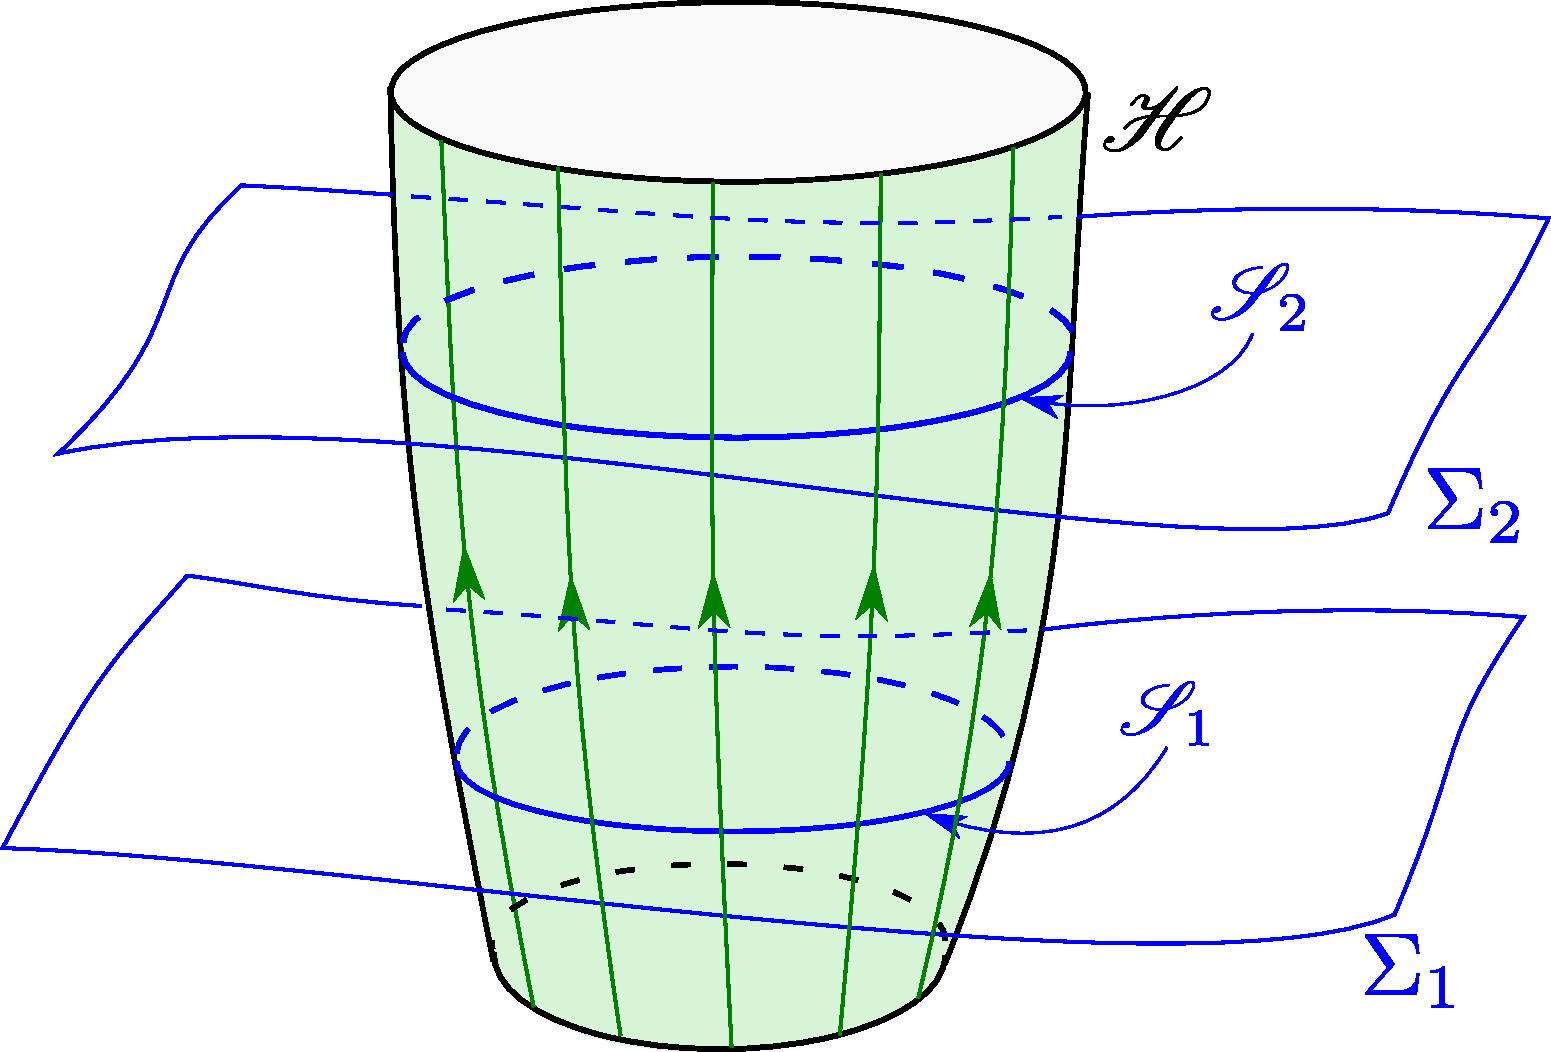
\includegraphics[width=0.6\textwidth]{evo_area_thm_smooth.pdf}}
\caption[]{\label{f:evo:area_thm_smooth} \footnotesize
Cross-sections $\Sp_1$ and $\Sp_2$ induced by the spacelike hypersurfaces $\Sigma_1$
and $\Sigma_2$ in a smooth part of the event horizon $\Hor$,
such that $\Sp_1$ and $\Sp_2$ are intersected by the same null geodesic
generators of $\Hor$ (green curves).}
\end{figure}



\begin{prop}[area theorem \textnormal{(Hawking\index[pers]{Hawking, S.W.} 1971 \cite{Hawki71},
Chru\'sciel\index[pers]{Chrusciel, P.T.@Chru\'sciel, P.T.},
Delay\index[pers]{Delay, E.},
Galloway\index[pers]{Galloway, G.J.} and Howard\index[pers]{Howard, R.} 2001
\cite{ChrusDGH01})}]
\label{p:evo:area_thm}
Let $(\M,\w{g})$ be a $n$-dimensional spacetime containing a black hole
of event horizon $\Hor$ and such that the Ricci tensor $\w{R}$ fulfills the null
energy condition (\ref{e:neh:null_energy_cond}), i.e.
$\w{R}(\wl, \wl) \geq 0$ for any null vector $\wl$.
Let $\Sigma_1$ and $\Sigma_2$ be spacelike hypersurfaces
such that $\Sigma_2$ lies in the causal future of $\Sigma_1$: $\Sigma_2\subset J^+(\Sigma_1)$
(cf. Sec.~\ref{s:glo:causal_struct}). Let $\Sp_1 = \Hor \cap \Sigma_1$
and $\Sp_2 = \Hor\cap\Sigma_2$.
If
\begin{itemize}
\item[(i)] $\Hor$ is smooth between $\Sp_1$ and $\Sp_2$ and $\Sp_1$ and $\Sp_2$
are cross-sections\footnote{If $\Hor$ is smooth between $\Sp_1$ and $\Sp_2$,
it is necessarily a null hypersurface there (Property~\ref{p:glo:prop4} on p.~\pageref{p:glo:prop4}),
so that the concept of cross-section as defined in Sec.~\ref{s:def:spacelike_sections}
makes sense.} of $\Hor$ that are intersected by the same null geodesic generators of $\Hor$
(cf. Fig.~\ref{f:evo:area_thm_smooth})
\end{itemize}
or
\begin{itemize}
\item[(ii)]
the closure of $J^-(\scri^+)\cup \Hor$ in
the conformal manifold $\tilde{\M}\supset\M$ defining $\scri^+$
is included in a globally hyperbolic
region $\mathscr{V}$ of $(\tilde{\M},\tilde{\w{g}})$
and $\Sigma_1$ and $\Sigma_2$ are Cauchy surfaces
of $\mathscr{V}$,
\end{itemize}
then the areas $A(\Sp_1)$ and $A(\Sp_2)$ obey
\be \label{e:evo:AS2_ge_AS1}
    A(\Sp_2) \geq A(\Sp_1) .
\ee
\end{prop}

\begin{figure}
\centerline{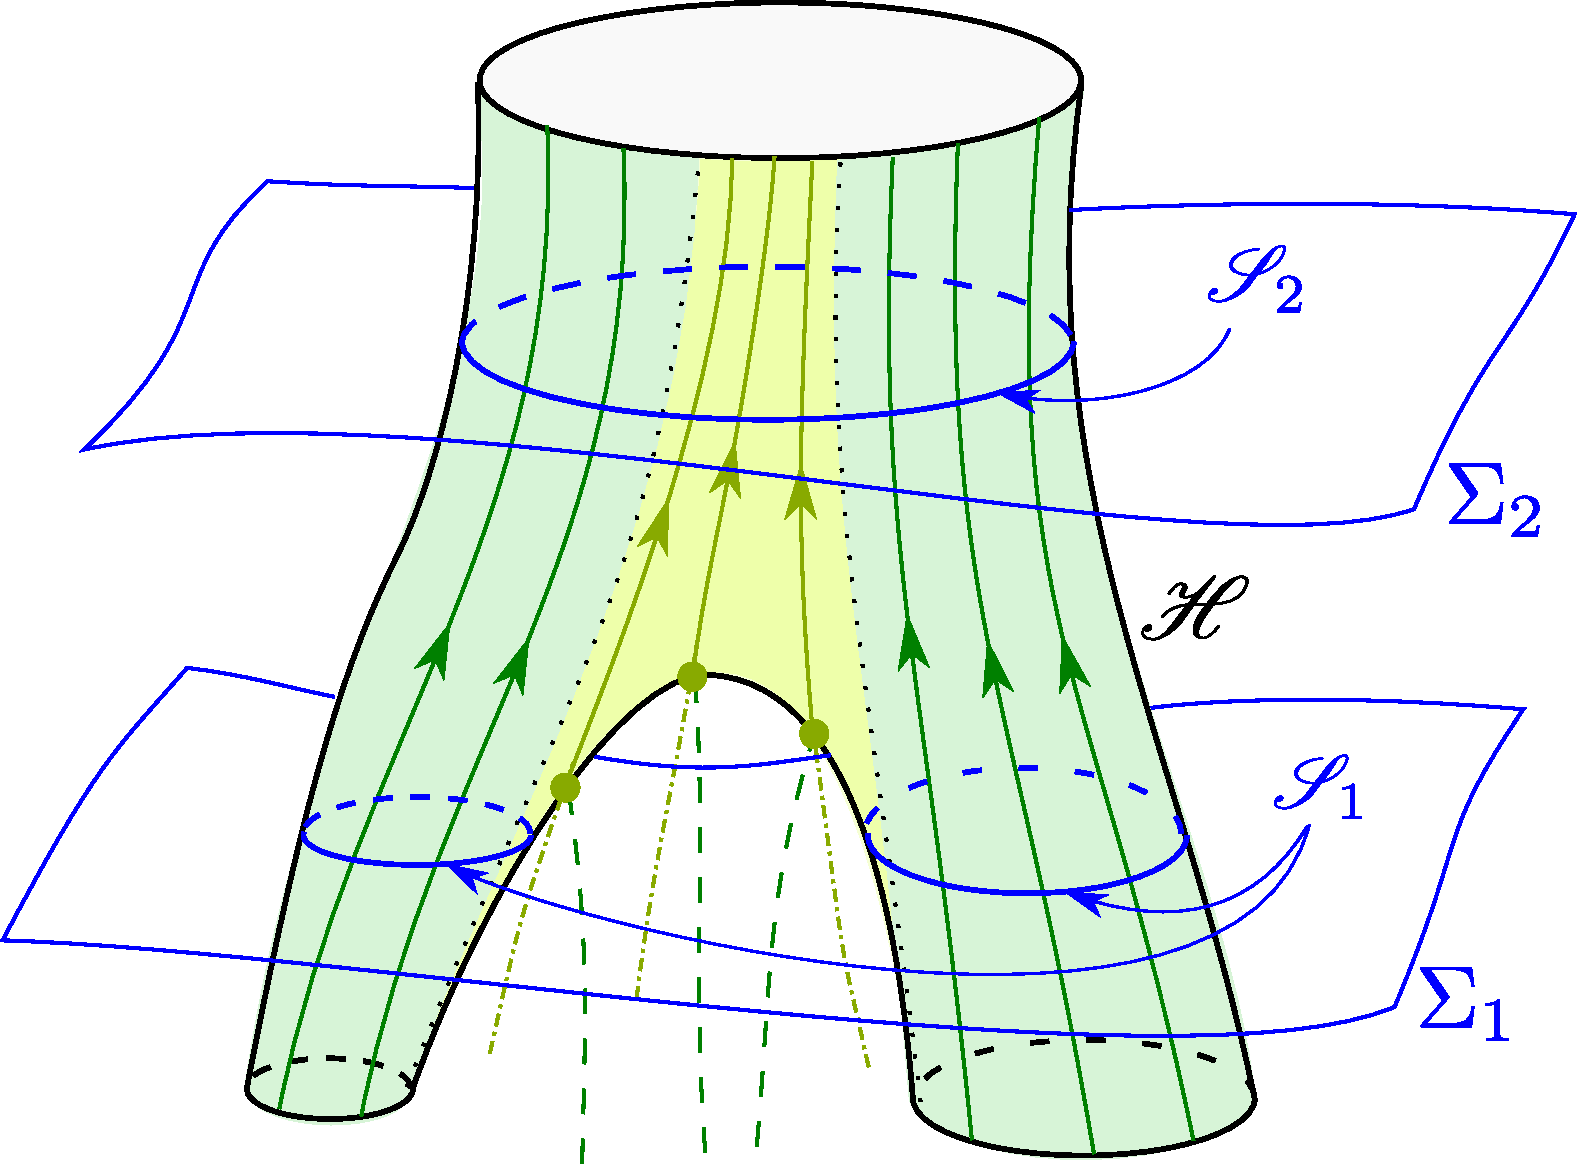
\includegraphics[width=0.6\textwidth]{evo_area_theorem.pdf}}
\caption[]{\label{f:evo:area_theorem} \footnotesize
Surfaces $\Sp_1$ and $\Sp_2$ induced by the spacelike hypersurfaces $\Sigma_1$
and $\Sigma_2$ on the event horizon $\Hor$ corresponding to a black hole merger.
All solid dark green and light green curves are null geodesic generators of $\Hor$.
The light green part of $\Hor$ is generated by null geodesics that
entered $\Hor$ at some caustic points (three of them are indicated as
light green dots); the parts of these geodesics outside $\Hor$ are drawn as
light green dot-dashed curves. The dark green dashed curves depict other null geodesics that
enter $\Hor$ at the same caustic points.}
\end{figure}


\begin{proof}
Let us consider first the case (i) ($\Hor$ smooth between
$\Sp_1$ and $\Sp_2$).
$\Sp_1$ and $\Sp_2$ are then cross-sections of $\Hor$
that are connected by null geodesic generators of $\Hor$
(cf. Fig.~\ref{f:evo:area_thm_smooth}).
One may introduce a 1-parameter foliation $(S_t)_{t\in [0,1]}$ of $\Hor$ by
cross-sections $S_t$ such that $S_0 = \Sp_1$ and $S_1 = \Sp_2$
(cf. the proof of Property~\ref{p:neh:invariance_area} for details, $\lambda$
playing the role of $t$ there). The label $t$
can then be considered as a parameter along the null geodesic generators of $\Hor$
connecting $\Sp_1$ to $\Sp_2$.
Let $\wl = \D\w{x}/\D t$ be the associated tangent vector.
Given that $\Sp_2$ lies in the future of $\Sp_1$, $\wl$ is future-directed.
By the very definition
of the expansion $\theta_{(\wl)}$ along $\wl$ [Eq.~(\ref{e:def:def_expansion})
combined with Eq.~(\ref{e:def:A_sqrt_q})], one has
\[
    \derd{}{t} A(S_t) = \int_{S_t} \theta_{(\wl)} \,  \sqrt{q} \, \D x^2 \cdots \D x^{n-1} ,
\]
where $(x^2, \ldots, x^{n-1})$ is a coordinate system on $S_t$ and $q$ is
the determinant with respect to these coordinates of the metric
induced by $\w{g}$ on $S_t$.
Now, if the null energy condition holds, Property~\ref{p:evo:positive_expansion} implies
$\theta_{(\wl)} \geq 0$; hence
\[
  \derd{}{t} A(S_t) \geq 0 .
\]
It follows that $t\mapsto A(S_t)$ is a nondecreasing function. Consequently, $A(S_1) \geq A(S_0)$
and Eq.~(\ref{e:evo:AS2_ge_AS1}) holds.

If $\Hor$ is not smooth between $\Sp_1$ and $\Sp_2$, this is due to the crease set\index{crease set},
i.e. the subset of $\Hor$ where new null geodesics enter $\Hor$ (cf. Sec.~\ref{s:glo:properties_H}).
Naively, this reinforces the inequality $A(\Sp_2) > A(\Sp_1)$ since the new geodesics
are generating new parts of $\Hor$ and therefore new parts of $\Sp_2$
with respect to those that can be connected to $\Sp_1$ by null geodesic generators
(cf. Fig.~\ref{f:evo:area_theorem}). More precisely, let us assume (ii) and
let us consider a point $p\in\Sp_1$. Let $\Li$ be the null geodesic
generator of $\Hor$ through $p$. By property~\ref{p:glo:prop3}, $\Li$ stays in $\Hor$ for all its future after $p$. Since $\Sigma_2$ is a Cauchy surface lying in the causal future of $\Sigma_1$, $\Li$
necessarily intersects $\Sigma_2$ at a unique point $q \in \Sigma_2\cap\Hor = \Sp_2$.
Hence every point of $\Sp_1$ is mapped to a point of $\Sp_2$ by a null geodesic generator.
Let $\Sp_2^*$ be the part of $\Sp_2$ covered by this map.
If we assume that the part of $\Hor$ between $\Sp_1$ and $\Sp_2^*$ is smooth,
we may apply (i) to the pair $(\Sp_1, \Sp_2^*)$
and get $A(\Sp_2^*) \geq A(\Sp_1)$. Given that $\Sp_2^* \subset \Sp_2$, one has
$A(\Sp_2) \geq A(\Sp_2^*)$ and (\ref{e:evo:AS2_ge_AS1}) follows.
We refer to the article \cite{ChrusDGH01} for the proof in the case where
$\Hor$ is not assumed smooth between $\Sp_1$ and $\Sp_2^*$ (70 pages!).
\end{proof}

\begin{example}[Oppenheimer-Snyder collapse]
Let us consider the black hole formed by the collapse
of a ball of pressureless matter, as described by the Oppenheimer-Snyder
model studied in Sec.~\ref{s:lem:OS}. Let $\Sp_{\ti}$ be a
cross-section of the event horizon at constant ingoing Eddington-Finkelstein coordinate $\ti$.
The area of $\Sp_{\ti}$ is simply $A = 4\pi r^2$,
where $r$ is the areal radius (cf. Sec.~\ref{s:lem:OS:BH_formation}). Its
evolution can thus be read directly on Fig.~\ref{f:lem:OS:diag_int_EF} (right):
it is increasing from $A = 0$ (at $\ti\simeq 5.6\, m$) to the Schwarzschild
value $A = 16\pi m^2$ (at $\ti\simeq 9.7\, m$). This fully agrees
with the area theorem, given that the null energy condition
is fulfilled by virtue of the Einstein equation (\ref{e:fra:Einstein_eq}) and the form
(\ref{e:lem:T_pressureless})
of the energy-momentum tensor of the collapsing matter: $\w{R}(\wl,\wl)
= 8\pi \w{T}(\wl,\wl) = 8\pi \rho (\w{u}\cdot\wl)^2 \geq 0$ since $\rho \geq 0$.
\end{example}

\begin{example}[Vaidya collapse]
Similarly, we check on Figs.~\ref{f:vai:diag_S0} and \ref{f:vai:diag_S2}
that for the radiation shell collapse studied in Chap.~\ref{s:vai},
the area of cross-sections of the event horizon
at constant ingoing Eddington-Finkelstein coordinate $t$
is increasing towards the future, for $r$ is again the areal radius
[cf. the metric (\ref{e:vai:metric_IEF})]. As we have already noticed in
Sec.~\ref{s:vai:general}, the radiation energy-momentum tensor (\ref{e:vai:ener_mom_tensor})
fulfills the null energy condition, given that $M'(v) \geq 0$ (cf. Fig.~\ref{f:vai:mass_function}).
\end{example}


\begin{hist}
The area theorem has been first established by Stephen Hawking\index[pers]{Hawking, S.W.}
in 1971 \cite{Hawki71} and a detailed proof was given in
Hawking \& Ellis' 1973 textbook (Proposition~9.2.7 in \cite{HawkiE73}).
In 2001, Piotr Chru\'sciel\index[pers]{Chrusciel, P.T.@Chru\'sciel, P.T.},
Erwann Delay\index[pers]{Delay, E.},
Gregory Galloway\index[pers]{Galloway, G.J.} and Ralph Howard\index[pers]{Howard, R.}
\cite{ChrusDGH01} pointed out that the Hawking \& Ellis proof is
valid only for $\Hor$ piecewise smooth (cf. the
discussion in Sec.~3.5.1 of Chru\'sciel's textbook \cite{Chrus20}) and constructed
a new proof that does not assume the smoothness of $\Hor$.
\end{hist}

\subsection{A second law?}

Basically the area theorem~\ref{p:evo:area_thm} states that
the area of cross-sections of a black hole event horizon
cannot decrease from the past to the future.
By its irreversible character, this property bears some resemblance
with the second law of thermodynamics.
By itself, this is of course not sufficient to identify the black hole area
with some entropy (any nondecaying physical quantity has not to be an entropy!).
However, we have seen in Sec.~\ref{s:evo:a_first_law_question} that the
candidate $T\D S$ term for a possible first law could be $\kappa/(8\pi)\D A$.
It is thus tempting to identify $A$ with some entropy $S$, up to some
constant factor $\alpha$. Then the temperature $T$ would be $\kappa/(8\pi\alpha)$:
\be \label{e:evo:identif_S_T}
    S = \alpha A \qand T = \frac{1}{8 \pi\alpha}\, \kappa ,
\ee
so that we get $T\D S = \kappa/(8\pi)\D A$, making
the mass variation formula (\ref{e:evo:mass_variation}) look pretty much like
the first law of thermodynamics.

%%%%%%%%%%%%%%%%%%%%%%%%%%%%%%%%%%%%%%%%%%%%%%%%%%%%%%%%%%%%%%%%%%%%%%%%%%%%%%%

\section{Zeroth and Third laws of black hole dynamics}

\subsection{Zeroth law}

We have already established a so-called \emph{zeroth law of black hole dynamics}
in Chap.~\ref{s:neh}: Property~\ref{p:neh:zeroth_law}, which states that
if the null dominant energy condition is fulfilled, the surface gravity
$\kappa$ of a Killing horizon is constant. Now, by Properties~\ref{p:sta:H_Killing_hor_xi_null}
and \ref{p:sta:strong_rigidity_thm}, (a connected component of) the event horizon
of a stationary black hole must be a Killing horizon. Hence, we may extend
the zeroth law to black holes\index{zeroth law of BH dynamics}:

\begin{prop}[zeroth law of black hole dynamics]
Let $(\M,\w{g})$ be a stationary spacetime of dimension $n\geq 4$ containing a black
hole. Let $\Hor$ be a connected component of the black hole event horizon.
If the null dominant energy condition [Eq.~(\ref{e:neh:null_dominant_cond})]
is fulfilled on $\Hor$ and under the hypotheses of
Property~\ref{p:sta:strong_rigidity_thm} if $\Hor$ is rotating
(i.e. if the stationary Killing vector $\w{\xi}$ is spacelike on some parts
of $\Hor$), then the surface gravity $\kappa$ is constant over $\Hor$.
\end{prop}

This property bears a strong resemblance with
the zeroth law of thermodynamics: the temperature of a body in equilibrium
is uniform over the entire body.
This strengthens the interpretation of the surface gravity
$\kappa$ as the temperature $T$ (up to some factor) performed in
Eq.~(\ref{e:evo:identif_S_T}).


\subsection{Third law}

%\begin{prop}[third law of black hole dynamics \textnormal{(Israel\index[pers]{Israel, W.} 1986 \cite{Israe86b})}]
%It is
%\end{prop}

%%%%%%%%%%%%%%%%%%%%%%%%%%%%%%%%%%%%%%%%%%%%%%%%%%%%%%%%%%%%%%%%%%%%%%%%%%%%%%%

\section{Black hole thermodynamics}

\subsection{The four laws}

\subsection{Hawking radiation and Bekenstein-Hawking entropy}
